% ====================================================================
% graphite_ica_ch1_v8-02.tex — Chapter 1 (v8-02: 유도 과정 포함 교과서 확장판)
%   베이스 = v7-11 (절 순서·결과박스·식별자·부호·표 보존).
%   확장   = v5 유도 원천에서 11식 유도 단계를 전부 복원(한줄 점프 금지).
%   그림   = v7-11 5개(그대로 또는 개선) + 신규 3개
%            (fig:gxi_derive: g(ξ) 이중웰·spinodal 유도 보조,
%             fig:lq_chain:  L_q 사슬 개요,
%             fig:fluxcross: 정·역 플럭스 교점 — v5 유래 개선).
%   빌드   = xelatex -interaction=nonstopmode 2-pass (kotex)
%   부호   = 브리프 §7 8항 전건 PASS (부호 사슬 §10 전수 검산).
% ====================================================================
\documentclass[11pt,a4paper]{article}
\usepackage[margin=22mm]{geometry}
\usepackage{kotex}
\setmonofont{D2Coding}[Scale=MatchLowercase]
\usepackage{amsmath,amssymb,mathtools,bm}
\usepackage{booktabs,longtable,array}
\usepackage{enumitem}
\usepackage{amsthm}
\usepackage{hyperref}
\usepackage{fancyhdr}
\usepackage{lastpage}
\usepackage{setspace}
\usepackage{tikz}
\usetikzlibrary{positioning,arrows.meta,calc,fit,backgrounds}
\setstretch{1.12}
\setlength{\parskip}{0.45em}\setlength{\parindent}{0pt}\setlength{\headheight}{14pt}
\setlength{\emergencystretch}{2em}
\hypersetup{colorlinks=true, linkcolor=blue, urlcolor=blue, citecolor=blue,
  pdftitle={흑연 음극 dQ/dV 이론: 코드 진행을 따라가는 교과서 확장판 — Chapter 1 (v8-02)}}
\pagestyle{fancy}\fancyhf{}
\lhead{흑연 음극 $dQ/dV$ 이론 — Ch.1 (v8-02, 유도 확장판)}\rhead{\thepage/\pageref{LastPage}}
\renewcommand{\headrulewidth}{0.4pt}

\newtheorem*{keybox}{핵심}
\newtheorem*{codebox}{코드 대응}
\newtheorem*{signbox}{부호 검산}
\newtheorem*{verifybox}{검산}
\newtheorem*{derivebox}{유도}

\newcommand{\dd}{\mathrm{d}}
\newcommand{\eff}{\mathrm{eff}}
\newcommand{\eq}{\mathrm{eq}}
\newcommand{\app}{\mathrm{app}}
\newcommand{\cell}{\mathrm{cell}}
\newcommand{\bg}{\mathrm{bg}}
\newcommand{\rxn}{\mathrm{rxn}}
\newcommand{\dis}{\mathrm{dis}}
\newcommand{\chg}{\mathrm{chg}}
\newcommand{\hys}{\mathrm{hys}}
\newcommand{\work}{\mathrm{work}}
\newcommand{\rep}{\mathrm{rep}}
\newcommand{\code}[1]{\texttt{#1}}

\renewcommand{\theequation}{1.\arabic{equation}}
\renewcommand{\thesection}{1.\arabic{section}}
\title{\textbf{\LARGE Chapter 1}\\[0.35em]\Large 흑연 음극 $dQ/dV$ 이론: 코드 진행을 따라가는 유도 확장판}
\author{}
\date{}

\makeatletter
\renewcommand*\l@section[2]{%
  \ifnum \c@tocdepth >\z@
    \addpenalty\@secpenalty
    \addvspace{1.0em \@plus\p@}%
    \setlength\@tempdima{2.3em}%
    \begingroup
      \parindent \z@ \rightskip \@pnumwidth
      \parfillskip -\@pnumwidth
      \leavevmode \bfseries
      \advance\leftskip\@tempdima
      \hskip -\leftskip
      #1\nobreak\hfil
      \nobreak\hb@xt@\@pnumwidth{\hss #2\kern-\p@\kern\p@}\par
    \endgroup
  \fi}
\renewcommand*\l@subsection{\@dottedtocline{2}{2.3em}{3.2em}}
\makeatother

\begin{document}
\maketitle

% ====================================================================
\section*{서론 — 이 문건이 따라가는 것}
\addcontentsline{toc}{section}{서론}
% ====================================================================
리튬이온전지 흑연 음극의 incremental capacity analysis(ICA)는 충방전 곡선 $Q(V)$ 의 미분
$\dd Q/\dd V$ 를 본다 \cite{bloom2005,dubarry2012}. 흑연은 staging 상전이(stage
$4\!\to\!3\!\to\!2\mathrm L\!\to\!2\!\to\!1$)를 거치며 \cite{dahn1991,ohzuku1993}, 각 전이 전위에서
두 상이 공존하면 전위가 거의 평탄해 좁은 $\dd V$ 에 큰 $\dd Q$ 가 몰려 $\dd Q/\dd V$ 가 치솟는다.

본 문건은 이 곡선을 \emph{한 번 그리는 계산}을 그대로 따라간다. 계산은 구현 \code{Anode\_Fit\_v11\_final.py}
의 메서드 \code{dqdv} 한 번 호출이며, 그 내부는 아홉 단계 $\mathrm N0\!\to\!\mathrm N9$ 를 순서대로 밟는다
(그림~\ref{fig:spine}). 각 절은 그 한 단계에서 코드가 평가하는 물리식을, \emph{출발 전제에서 결과 박스까지} 빠짐없이
유도한다. 도착점은 한 줄 합산식과, ``이 문건만 보고 같은 곡선을 재현하는 코드를 짤 수 있다''는 실행 가능성이다.

\textbf{관측.}
\begin{quote}\itshape
$\dd Q/\dd V$ 상전이 peak 의 위치$\cdot$너비$\cdot$높이는 (a) 온도 $T$, (b) 극판 전위, (c) C-rate(전류)
세 가지에 따라 변한다. 저온$\cdot$고율일수록 peak 의 꼬리가 길어져 다음 peak 와 겹치고, 같은 전이가 충전과 방전에서
서로 다른 전위에 peak 를 남기며(충방전 히스테리시스), 이 갈림에는 전류를 $0$ 으로 줄여도 사라지지 않는 성분이 있다.
\end{quote}

세 인자는 모두 하나의 속도식 $k\simeq k_0\exp[-\Delta G_a/RT]$ 의 서로 다른 자리로 들어온다 — 온도는 지수의 분모,
전위는 장벽 $\Delta G_a$ 자체, C-rate 는 요구 속도와 공급 속도의 경쟁이다. 코드 진행이 이 세 갈래를 차례로 닫는다.

\begin{figure}[t]
\centering
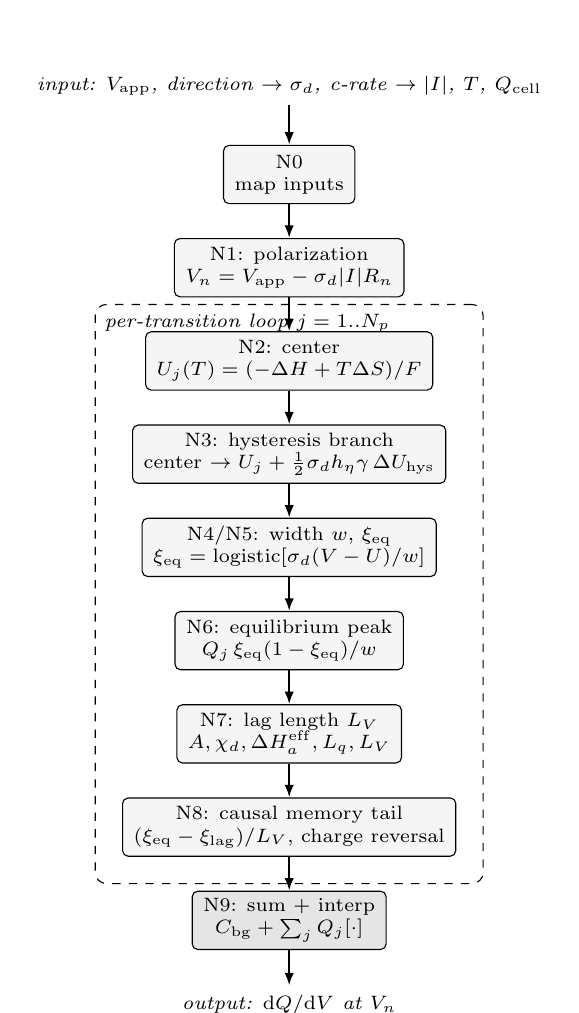
\begin{tikzpicture}[
  node distance=4.3mm and 5.5mm,
  stage/.style={draw,rounded corners=2pt,minimum height=7.4mm,inner xsep=4pt,inner ysep=2.5pt,font=\scriptsize,align=center,fill=black!4},
  core/.style={stage,fill=black!10},
  io/.style={font=\scriptsize\itshape,align=center},
  ar/.style={-{Latex[length=1.6mm]},thick}]
\node[io] (in) {input: $V_\app$, direction $\to\sigma_d$, c-rate $\to|I|$, $T$, $Q_\cell$};
\node[stage,below=5mm of in] (n0) {N0\\map inputs};
\node[stage,below=of n0] (n1) {N1: polarization\\$V_n=V_\app-\sigma_d|I|R_n$};
\node[stage,below=of n1] (n2) {N2: center\\$U_j(T)=(-\Delta H+T\Delta S)/F$};
\node[stage,below=of n2] (n3) {N3: hysteresis branch\\center $\to U_j+\tfrac12\sigma_d h_\eta\gamma\,\Delta U_\hys$};
\node[stage,below=of n3] (n4) {N4/N5: width $w$, $\xi_\eq$\\$\xi_\eq=\mathrm{logistic}[\sigma_d(V-U)/w]$};
\node[stage,below=of n4] (n6) {N6: equilibrium peak\\$Q_j\,\xi_\eq(1-\xi_\eq)/w$};
\node[stage,below=of n6] (n7) {N7: lag length $L_V$\\$A,\chi_d,\Delta H_a^\eff,L_q,L_V$};
\node[stage,below=of n7] (n8) {N8: causal memory tail\\$(\xi_\eq-\xi_\mathrm{lag})/L_V$, charge reversal};
\node[core,below=of n8] (n9) {N9: sum + interp\\$C_\bg+\sum_j Q_j[\cdot]$};
\node[io,below=4.5mm of n9] (out) {output: $\dd Q/\dd V$ at $V_n$};
\foreach \a/\b in {in/n0,n0/n1,n1/n2,n2/n3,n3/n4,n4/n6,n6/n7,n7/n8,n8/n9,n9/out}
  \draw[ar] (\a) -- (\b);
\begin{scope}[on background layer]
\node[draw,dashed,rounded corners,fit=(n2)(n3)(n4)(n6)(n7)(n8),inner sep=3.4mm,
  label={[font=\scriptsize\itshape,anchor=north west]north west:per-transition loop $j=1..N_p$}] (loop) {};
\end{scope}
\end{tikzpicture}
\caption{한 곡선을 그리는 코드 진행(spine). 외부 실험조건이 \code{curve} facade 에서 $(\sigma_d,|I|,T,Q_\cell)$
로 환산($\mathrm N0$)되어 코어 \code{dqdv} 로 들어가고, 분극으로 내부 전위 $V_n$ 을 얻은 뒤($\mathrm N1$),
전이 $j$ 마다 평형 중심$\cdot$히스 분기$\cdot$폭$\cdot$평형 점유$\cdot$평형 peak$\cdot$지연 길이$\cdot$인과 꼬리를
계산해($\mathrm N2$--$\mathrm N8$) 합산$\cdot$역보간한다($\mathrm N9$). 본 문건의 절 번호가 이 노드 순서다.
점선 상자가 코드의 전이 루프(\code{for tr in transitions}).}
\label{fig:spine}
\end{figure}

\tableofcontents
\newpage

% ====================================================================
\section{기호와 규약, 실험조건 매핑 (N0)}\label{sec:notation}
% ====================================================================
계산의 진입점은 facade \code{curve}$(V_\app,\text{direction},\text{c\_rate},Q_\cell,T)$ 이고, 그 첫 일은 실험조건을
코어 \code{dqdv} 의 모델 입력으로 환산하는 것이다 — 이것이 노드 $\mathrm N0$ 다. 방향 문자열은 방향 부호 $\sigma_d$ 로,
C-rate 는 전류 크기 $|I|$ 로 바뀐다:
\begin{equation}
\sigma_d=\begin{cases}+1 & \text{방전(discharge)}\\ -1 & \text{충전(charge)}\end{cases},
\qquad
|I|=\text{c\_rate}\cdot Q_\cell\quad(\text{또는 }I_\mathrm{abs}\text{ 직접 지정}).
\label{eq:n0map}
\end{equation}
방향 부호의 작용처는 셋 — 분극 부호($\mathrm N1$), 분기 중심 선택($\mathrm N3$), 꼬리 지지 방향($\mathrm N8$) — 이며,
평형 종 자체는 방향 불변이다. 본 장이 뽑는 양은 $\dd Q/\dd V$ 한 곡선이다.

\textbf{전이 인덱스.} $j=1,\dots,N_p$($N_p\approx3$--$4$). 전이 $j$ 의 진행률 $\xi_j$(방전 시 $0\to1$ 로 증가, 탈리튬화 진행),
용량 가중 $Q_j$. 박스 결과식은 $j$ 첨자를 단다.

\textbf{부호 규약(★최우선 결함 클래스).} 전위는 흑연 음극 반쪽전지 전위(vs Li/Li$^+$)다. 방향 부호 $\sigma_d=\pm1$
(방전 $+1$/충전 $-1$)이 코드의 \code{s} 인자이며, 평형 점유 $\xi_\eq=\mathrm{logistic}[\sigma_d(V-U)/w]$ 에서 방전
($\sigma_d=+1$)은 $V\!\uparrow\Rightarrow\xi_\eq\!\uparrow$(전위를 올리면 탈리튬화). 분기 중심 $\pm\tfrac12\sigma_d(\cdots)$
는 방전$\cdot$충전이 반대로 갈리고, 꼬리는 충전에서 격자 역전을 받는다.

\begin{longtable}{p{0.17\textwidth} p{0.16\textwidth} p{0.585\textwidth}}
\toprule 기호(코드 식별자) & 단위 & 의미 \\ \midrule \endhead
\multicolumn{3}{l}{\emph{— 실험조건$\cdot$방향(N0$\cdot$N1) —}}\\
$\sigma_d$ (\code{s},\,\code{sigma\_d}) & --- & 방향 부호 — 방전 $+1$/충전 $-1$ \\
$|I|$ (\code{I\_abs}) & A & 전류 크기 $=$ c\_rate$\cdot Q_\cell$ \\
$Q_\cell$ (\code{Q\_cell}) & C & 셀 용량(전하) \\
$T$ (\code{T}) & K & 온도 \\
$R_n$ (\code{Rn}) & $\Omega$ & 음극 lumped 분극 저항 \\
$V_\app$ (\code{V\_app}) & V & 인가(측정) 전위 격자 \\
$V_n$ & V & 내부(열역학) 전위 $=V_\app-\sigma_d|I|R_n$ \\
\multicolumn{3}{l}{\emph{— 평형 중심$\cdot$폭$\cdot$점유(N2$\cdot$N4$\cdot$N5) —}}\\
$U_j(T)$ (\code{U},\,\code{func\_U\_j}) & V & 전이 $j$ 평형 중심 전위 $=(-\Delta H_{\rxn,j}+T\Delta S_{\rxn,j})/F$ \\
$\Delta H_{\rxn,j},\Delta S_{\rxn,j}$ (\code{dH\_rxn},\code{dS\_rxn}) & {\footnotesize J/mol;\,J/(mol\,K)} & 삽입 반응 엔탈피$\cdot$엔트로피 \\
$n_j$ (\code{n}) & --- & 폭 다중도($w=n_jRT/F$) \\
$w_j$ (\code{func\_w}) & V & 전이 폭 척도 $=n_jRT/F$ \\
$\xi_{\eq,j}$ (\code{func\_ksi\_eq}) & --- & 평형 진행률(logistic) \\
$Q_j$ (\code{Q}) & C & 전이 $j$ 용량 가중 \\
$C_\bg$ (\code{Cbg}) & C/V & 배경 미분용량 \\
\multicolumn{3}{l}{\emph{— 히스테리시스 분기(N3) —}}\\
$\Omega_j$ (\code{Omega}) & J/mol & 정규용액 상호작용 에너지($>2RT$ 면 상분리) \\
$\gamma_j$ (\code{gamma}) & --- & 분기 축소 인자 $0\le\gamma_j\le1$ \\
$\Delta U_j^\hys$ (\code{func\_dU\_hys}) & V & spinodal 상한 분기 gap \\
$h_{\eta,j}$ (\code{h\_eta}) & --- & 부분 cycle 인자(기본 $1$) \\
$U_j^{\,d}$ (\code{center}) & V & 방향별 분기 중심 \\
\multicolumn{3}{l}{\emph{— 동역학 꼬리(N7$\cdot$N8) —}}\\
$\chi$ (\code{chi}) & --- & 전이상태 분율 위치(전달 계수) \\
$\chi_d$ (\code{func\_chi\_d}) & --- & 방향별 전달 계수 — 방전 $\chi$/충전 $1-\chi$ \\
$\mathcal A$ (\code{A}) & J/mol & 꼬리 컷점 affinity \\
$\Delta H_{a,j},\Delta S_{a,j}$ (\code{dH\_a},\code{dS\_a}) & {\footnotesize J/mol;\,J/(mol\,K)} & 활성화 엔탈피$\cdot$엔트로피 \\
$\Delta H_{a,j}^\eff$ (\code{func\_dH\_a\_eff}) & J/mol & 유효 장벽 $=\Delta H_a-\chi_d\Omega$ \\
$L_{q,j}$ (\code{func\_L\_q}) & --- & 용량축 지연 길이 \\
$L_{V,j}$ (\code{lag\_len\_V}) & V & 전압축 지연 길이 $=|\dd V/\dd q|_{q_a}L_{q,j}$ \\
$z_\mathrm{cut}$ (\code{z\_cut}) & --- & 컷 affinity 의 $z=\mathcal A/(n_jRT)$(기본 $4.357$) \\
$A_\mathrm{cap}$ (\code{A\_cap\_RT}) & --- & 컷 affinity 상한 배수(기본 $4.0$) \\
$\xi_{\mathrm{lag},j}$ (\code{occ\_lagged}) & --- & 인과 저역통과된 진행률 \\
\multicolumn{3}{l}{\emph{— 상수 —}}\\
$R,F,k_B,h$ & {\footnotesize J/(mol\,K), C/mol, J/K, J\,s} & 기체상수, Faraday, Boltzmann, Planck \\
\bottomrule
\end{longtable}

흑연 staging 의 갤러리 채움을 그림~\ref{fig:staging} 에 둔다.

\begin{figure}[t]
\centering
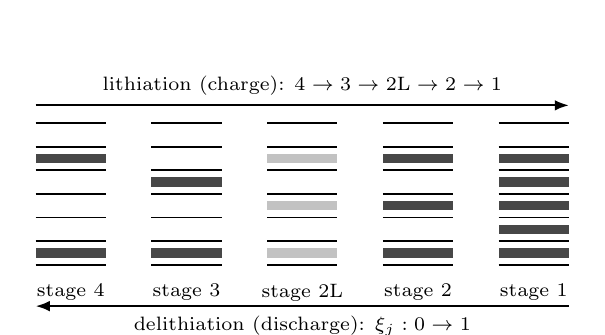
\begin{tikzpicture}[x=1.05cm,y=0.5cm,
  lab/.style={font=\scriptsize,align=center},
  fill4/.style={fill=black!72},fillL/.style={fill=black!24}]
\def\colw{0.85}
\foreach \x/\name/\style in {0/{stage 4}/fill4, 1.4/{stage 3}/fill4, 2.8/{stage 2L}/fillL, 4.2/{stage 2}/fill4, 5.6/{stage 1}/fill4}{
  \draw[semithick] (\x,0)--(\x+\colw,0);
  \foreach \k in {1,2,3,4,5,6}{\draw[semithick] (\x,0.6*\k)--(\x+\colw,0.6*\k);}
  \node[lab,below] at (\x+\colw/2,-0.25) {\name};
}
\foreach \k in {1,5}{\fill[black!72] (0,0.6*\k-0.42) rectangle (0+\colw,0.6*\k-0.18);}
\foreach \k in {1,4}{\fill[black!72] (1.4,0.6*\k-0.42) rectangle (1.4+\colw,0.6*\k-0.18);}
\foreach \k in {1,3,5}{\fill[black!24] (2.8,0.6*\k-0.42) rectangle (2.8+\colw,0.6*\k-0.18);}
\foreach \k in {1,3,5}{\fill[black!72] (4.2,0.6*\k-0.42) rectangle (4.2+\colw,0.6*\k-0.18);}
\foreach \k in {1,2,3,4,5}{\fill[black!72] (5.6,0.6*\k-0.42) rectangle (5.6+\colw,0.6*\k-0.18);}
\draw[-{Latex[length=1.8mm]},thick] (0,4.05)--(6.45,4.05) node[pos=0.5,above,font=\scriptsize] {lithiation (charge): $4\to3\to2\mathrm L\to2\to1$};
\draw[{Latex[length=1.8mm]}-,thick] (0,-1.05)--(6.45,-1.05) node[pos=0.5,below,font=\scriptsize] {delithiation (discharge): $\xi_j:0\to1$};
\end{tikzpicture}
\caption{흑연 staging 의 갤러리 채움 도식(v7-11 개선). 수평선이 그래핀 층, 음영 띠가 리튬이 든 층간 갤러리다.
채울수록 stage 번호가 줄어 stage 1($\mathrm{LiC_6}$)에 닿고, 각 stage 전이가 $\dd Q/\dd V$ 에 peak 하나를 남긴다.
방전은 탈리튬화 방향(진행률 $\xi_j:0\to1$)이다.}
\label{fig:staging}
\end{figure}

% ====================================================================
\section{분극 — 측정 전위에서 내부 전위로 (N1)}\label{sec:pol}
% ====================================================================
코어 \code{dqdv} 의 첫 식은 분극을 벗기는 환산이다. 관측은 유한 전류에서 이루어지므로 측정 전위 $V_\app$ 에는 셀의
직렬 저항을 통과한 IR 분극이 실려 있고, 평형 열역학이 사는 전위는 그 분극을 벗긴 내부 전위 $V_n$ 이다.

\subsection{분극 부호 — 방향이 결정한다}
전류 크기 $|I|$ 가 lumped 저항 $R_n$ 을 통과하며 만드는 전위 강하가 $|I|R_n$ 이고, 그 부호는 전류 방향이 정한다.
방전($\sigma_d=+1$)은 음극에서 산화(탈리튬화)가 일어나는 방향이라 측정 전위가 내부 전위보다 분극만큼 \emph{높게}
관측되므로, 내부 전위는 그만큼 낮춰 읽어야 한다. 충전($\sigma_d=-1$)은 부호가 반대다. 두 경우를 한 식으로 묶으면
\begin{equation}
\boxed{\;V_n\;=\;V_\app\;-\;\sigma_d\,|I|\,R_n\;.}
\label{eq:vn}
\end{equation}
이것이 코드의 \code{V\_n = V\_in - sigma\_d * I\_abs * self.Rn} 한 줄이다. 방전에서 $V_n=V_\app-|I|R_n<V_\app$(측정이 내부보다 높음), 충전에서 $V_n=V_\app+|I|R_n>V_\app$, $|I|\to0$ 또는 $R_n=0$ 에서 $V_n=V_\app$ 다.

\subsection{작업 격자 — 꼬리가 들어올 여유}
이후 모든 전이 계산은 $V_n$ 의 범위를 양쪽으로 넓힌 균일 \emph{작업 격자} $V_\work$ 위에서 이루어진다.
$v_\mathrm{lo}=\min V_n$, $v_\mathrm{hi}=\max V_n$, $\Delta v=v_\mathrm{hi}-v_\mathrm{lo}$ 로
\begin{equation}
V_\work=\mathrm{linspace}\big(v_\mathrm{lo}-p_\mathrm{lo}\,\Delta v,\;
v_\mathrm{hi}+p_\mathrm{hi}\,\Delta v,\;n_\work\big),
\qquad \Delta_\mathrm{grid}=V_{\work,1}-V_{\work,0},
\label{eq:vwork}
\end{equation}
패딩 $p_\mathrm{lo}=p_\mathrm{hi}=0.15$, 점 수 $n_\work=\max(2048,\,2\,|V_n|)$ 이다. 배경은 작업 격자 위에서 먼저 깔린다:
$\dd Q/\dd V|_\work \leftarrow C_\bg(V_\work)$. 모든 전이 기여는 여기에 더해지고($\mathrm N9$), 마지막에 $V_n$ 으로
역보간된다.

\begin{keybox}
\textbf{세 전위.} $V_\app$(측정)$\cdot$$V_n$(내부, 식~\eqref{eq:vn})$\cdot$$V_\work$(계산 격자, 식~\eqref{eq:vwork})는
지위가 다르다. 다음 절부터 평형$\cdot$동역학은 $V_\work$ 위에서 풀고, 출력만 $V_n$ 으로 되돌린다.
\end{keybox}

다음 절은 전이 루프의 첫 식 — 평형 중심 $U_j(T)$ — 으로 들어간다.

% ====================================================================
\section{평형 중심 $U_j(T)$ — 열역학에서 (N2)}\label{sec:center}
% ====================================================================
전이 루프 안의 첫 물리량은 전이 $j$ 의 평형 중심 전위 $U_j(T)$ 다.
이 절은 그 환산식이 Gibbs 자유에너지와 전기화학 평형에서 어떻게 나오는지를 단계별로 닫는다.

\subsection{$G$, $\mu$ 와 전기화학 평형 — 출발 전제}

등온$\cdot$등압 계(전지)의 자발성을 판정하는 퍼텐셜은 Gibbs 자유에너지다:
\begin{equation}
G\;\equiv\;H-TS.
\label{eq:gibbsdef}
\end{equation}
입자 1몰 변화당 $G$ 변화가 화학퍼텐셜이다:
\begin{equation}
\mu\;\equiv\;\frac{\partial G}{\partial n}\Big|_{T,P}.
\label{eq:mudef}
\end{equation}
삽입 반응 $\mathrm{Li}^++e^-+[\,]\rightleftharpoons\mathrm{Li}_{(\text{흑연})}$ 에서, 전자 항이 반쪽전지 전위 $V$ 를 통해
$-FV$ 로 들어오므로 전기화학 평형 조건은 두 골짜기 화학퍼텐셜이 같아지는 조건 $\delta G=0$ 에서 나온다. 반응의 자유에너지 변화는
\begin{equation}
\Delta G_j\;=\;\mu_{\mathrm{Li}}(\xi_{\eq,j})-\mu^0_{\mathrm{Li}^+}-\mu^0_{e^-}+FV.
\label{eq:dGdef}
\end{equation}
전해질$\cdot$준위 상수(온도 $T$ 에서 고정)를 묶어 $\Delta G_j^0\equiv\mu^0_{\mathrm{Li}^+}+\mu^0_{e^-}-\mu^0_{\mathrm{Li}}$ 로 정의하면, 평형($\Delta G_j=0$)에서
\begin{equation}
FV_{\eq}=\Delta G_j^0\quad\Longrightarrow\quad \Delta G_j=-F(V-V_{\eq})\equiv-sF(V-U_j),
\label{eq:eqcond}
\end{equation}
즉 $\Delta G_j=-sFU_j$ 의 지위($s=+1$ 방전 규약)다. 부호의 핵심 — $U_j>0$ 이면 $\Delta G_j<0$(자발), 전이 중심에서 두 골짜기가 같은 높이다.

\subsection{$U_j(T)$ 의 유도 — $\Delta G = \Delta H - T\Delta S$ 대입}

\begin{derivebox}
\textbf{출발.} 삽입 반응의 반응 자유에너지 $\Delta G_j=\Delta H_{\rxn,j}-T\Delta S_{\rxn,j}$ 를 평형 조건 식~\eqref{eq:eqcond} 의 $\Delta G_j=-sF\,U_j$($s=+1$)에 대입한다.

\textbf{대입.}
\begin{equation*}
\Delta H_{\rxn,j}-T\Delta S_{\rxn,j}\;=\;-F\,U_j.
\end{equation*}

\textbf{$U_j$ 로 풀기.} 양변을 $(-F)$ 로 나눈다:
\begin{equation*}
U_j\;=\;\frac{-(\Delta H_{\rxn,j}-T\Delta S_{\rxn,j})}{F}.
\end{equation*}

\textbf{정리.}
\end{derivebox}
\begin{equation}
\boxed{\;U_j(T)\;=\;\frac{-\Delta H_{\rxn,j}+T\,\Delta S_{\rxn,j}}{F}\;.}
\label{eq:Uj}
\end{equation}
이것이 \code{func\_U\_j(T, dH\_rxn, dS\_rxn)} 의 \code{(-dH\_rxn + T*dS\_rxn)/F} 다. 부호 — 발열 반응
$\Delta H_\rxn<0$ 이면 분자 $-\Delta H_\rxn>0$ 이 중심을 \emph{올린다}. 온도 의존은
$\partial U_j/\partial T=\Delta S_{\rxn,j}/F$ 이고, $|\Delta S_\rxn|\sim$ 수 J/(mol\,K) 라 $30$ K 창에서 수 mV
규모로 중심이 이동한다.

\begin{codebox}
\textbf{N2.} \code{if 'dH\_rxn' in tr: U\_j = func\_U\_j(T\_work, dH\_rxn, dS\_rxn)}
— 배열 $T_\work$ 대응. 없으면 \code{U\_j = float(tr['U'])} 직접. 예: stage $2\!\to\!1$,
$\Delta H_\rxn=-13000$ J/mol, $\Delta S_\rxn=-16$ J/(mol\,K) $\Rightarrow$ $U(298)=(13000-298\times16)/96485
\approx0.0853$ V.
\end{codebox}

다음은 같은 루프 안에서 이 중심을 충$\cdot$방전으로 갈라놓는 히스테리시스 분기다.

% ====================================================================
\section{히스테리시스 분기 중심 (N3)}\label{sec:hys}
% ====================================================================
코드는 평형 중심 $U_j$ 를 곧바로 쓰지 않고, 상호작용 $\Omega_j$ 와 분기 인자 $\gamma_j$ 가 있으면 방향별 분기 중심
$U_j^{\,d}$ 로 옮긴다. 이 절은 그 gap 의 닫힌 식과 부호를 자유에너지 $g_j(\xi)$ 에서 단계별로 유도한다.

\subsection{정규용액 자유에너지 $g_j(\xi)$ — 출발 전제}

흑연 격자기체의 1몰당 잉여 자유에너지를 진행률 $\xi=1-\theta$ 로 적으면 세 몫으로 분해된다:

\begin{derivebox}
\textbf{(i) 섞임 엔트로피 몫.} $N$ 자리 중 $n=N\xi$ 를 고르는 경우의 수 $W=\binom{N}{N\xi}$ 에 Stirling 근사를 적용하면
$S_\mathrm{mix}/N_A=R[\xi\ln\xi+(1-\xi)\ln(1-\xi)]$ 이므로, 온도 가중 몫은 $RT[\xi\ln\xi+(1-\xi)\ln(1-\xi)]$.

\textbf{(ii) 상호작용 몫.} 점유 이웃 쌍의 평균장 에너지를 정리하면 $\Omega_j\xi(1-\xi)$ ($\Omega_j>0$: 동종 인력).

\textbf{(iii) 합산.} 기준 잔여(선형 몫은 공통 접선 판정에 불변이라 제거 가능)를 $g_j^0$ 로 묶으면
\end{derivebox}
\begin{equation}
g_j(\xi)=g_j^0+RT\big[\xi\ln\xi+(1-\xi)\ln(1-\xi)\big]+\Omega_j\,\xi(1-\xi).
\label{eq:gxi}
\end{equation}

그림~\ref{fig:gxi_derive} 가 $g_j(\xi)$ 의 형태와 spinodal 경계를 보인다.

\begin{figure}[t]
\centering
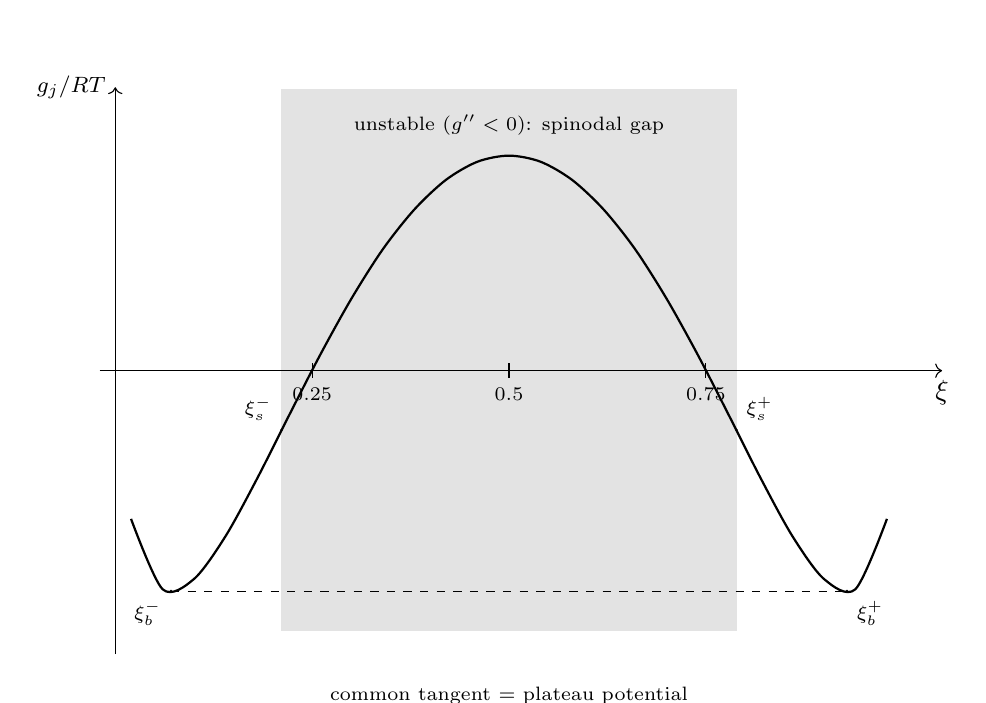
\begin{tikzpicture}[x=10cm,y=48cm]
% shading: spinodal region (xi in [0.211,0.789] for Omega=3RT)
\fill[gray!22] (0.211,-0.069) rectangle (0.789,0.0745);
\draw[->] (0,-0.075) -- (0,0.075) node[left] {\footnotesize $g_j/RT$};
\draw[->] (-0.02,0) -- (1.05,0) node[below] {$\xi$};
\foreach \xx in {0.25,0.5,0.75} {\draw (\xx,0.002) -- (\xx,-0.002) node[below] {\scriptsize $\xx$};}
% g(xi) for Omega=3RT (double-well)
\draw[thick] plot[smooth] coordinates {
  (0.02,-0.0392)(0.06,-0.0578)(0.1,-0.0551)(0.14,-0.0438)(0.18,-0.0286)
  (0.22,-0.0121)(0.26,0.0041)(0.3,0.0191)(0.34,0.0322)(0.38,0.0427)
  (0.42,0.0505)(0.46,0.0553)(0.5,0.0569)(0.54,0.0553)(0.58,0.0505)
  (0.62,0.0427)(0.66,0.0322)(0.7,0.0191)(0.74,0.0041)(0.78,-0.0121)
  (0.82,-0.0286)(0.86,-0.0438)(0.9,-0.0551)(0.94,-0.0578)(0.98,-0.0392)};
% common tangent (binodal)
\draw[dashed] (0.0707,-0.0583) -- (0.9293,-0.0583);
\fill (0.0707,-0.0583) circle (0.5pt) node[below left] {\scriptsize $\xi_b^-$};
\fill (0.9293,-0.0583) circle (0.5pt) node[below right] {\scriptsize $\xi_b^+$};
% spinodal points (inflection)
\fill (0.211,-0.0157) circle (0.5pt) node[above left] {\scriptsize $\xi_s^-$};
\fill (0.789,-0.0157) circle (0.5pt) node[above right] {\scriptsize $\xi_s^+$};
\node at (0.5,0.065) {\scriptsize unstable ($g''<0$): spinodal gap};
\node[below] at (0.0707,-0.063) {};
\node at (0.5,-0.086) {\scriptsize common tangent $=$ plateau potential};
\end{tikzpicture}
\caption{정규용액 자유에너지~\eqref{eq:gxi}($\Omega_j=3RT$; 신규). 이중웰 구조에서 공통 접선(파선) 접점이 binodal $\xi_b^\pm$,
변곡점이 spinodal $\xi_s^\pm$(식~\eqref{eq:spinodal}). 음영 띠($g''<0$)에서 즉시 상분리, 그 밖 준안정 — 과주행 히스테리시스의 무대.
스피노달 경계 $\xi_s^\pm=\tfrac12(1\pm u)$ 가 $\Delta U_j^\hys$ 유도의 시작점이다.}
\label{fig:gxi_derive}
\end{figure}

\subsection{spinodal 의 유도 — $g_j''=0$ 의 근}

\begin{derivebox}
\textbf{출발.} 식~\eqref{eq:gxi} 를 두 번 미분한다.

\textbf{1차 미분.}
\begin{equation*}
g_j'(\xi)=RT\Big[\ln\xi+1-\ln(1-\xi)-1\Big]+\Omega_j(1-2\xi)
=RT\ln\frac{\xi}{1-\xi}+\Omega_j(1-2\xi).
\end{equation*}
(로그 항 미분에서 $+1$과 $-1$이 상쇄된다.)

\textbf{2차 미분.}
\begin{equation*}
g_j''(\xi)=RT\Big[\frac{1}{\xi}+\frac{1}{1-\xi}\Big]-2\Omega_j
=\frac{RT}{\xi(1-\xi)}-2\Omega_j.
\end{equation*}

\textbf{$g_j''=0$ 설정 및 전개.}
\begin{equation*}
\frac{RT}{\xi(1-\xi)}=2\Omega_j
\;\Longrightarrow\;
\xi(1-\xi)=\frac{RT}{2\Omega_j}
\;\Longrightarrow\;
\xi^2-\xi+\frac{RT}{2\Omega_j}=0.
\end{equation*}

\textbf{근의 공식 적용.}
\begin{equation*}
\xi=\frac{1\pm\sqrt{1-4\cdot\frac{RT}{2\Omega_j}}}{2}
=\frac{1\pm\sqrt{1-\frac{2RT}{\Omega_j}}}{2}.
\end{equation*}
\end{derivebox}
\begin{equation}
\xi_{s,j}^\pm=\tfrac12(1\pm u_j),\qquad
u_j\equiv\sqrt{1-\frac{2RT}{\Omega_j}}\quad(\Omega_j>2RT).
\label{eq:spinodal}
\end{equation}
$u_j$ 가 실수가 되는 조건 $\Omega_j>2RT$ 가 상분리(따라서 히스테리시스)의 문턱이다.

\subsection{$\Delta U_j^\hys$ 의 유도 — 두 spinodal 에서의 전위 차}

평형 전위 곡선은 $g_j'(\xi)=sF(V_{\eq,j}-U_j)$ 에서 나온다. $s=+1$ 로 두면
\begin{equation}
V_{\eq,j}(\xi)=U_j+\frac{1}{F}\Big[RT\ln\frac{\xi}{1-\xi}+\Omega_j(1-2\xi)\Big].
\label{eq:Veq}
\end{equation}

\begin{derivebox}
\textbf{방전은 $\xi_{s,j}^-$ 까지, 충전은 $\xi_{s,j}^+$ 까지 과주행한다}(그림~\ref{fig:hysloop}).

\textbf{각 spinodal 에서의 전위 계산.}

$\xi=\xi_{s,j}^-=\tfrac12(1-u_j)$ 에서: $(1-2\xi_{s}^-)=1-(1-u_j)=+u_j$,
$\xi_{s}^-/(1-\xi_{s}^-)=[1-u_j]/[1+u_j]$.

$\xi=\xi_{s,j}^+=\tfrac12(1+u_j)$ 에서: $(1-2\xi_{s}^+)=1-(1+u_j)=-u_j$,
$\xi_{s}^+/(1-\xi_{s}^+)=[1+u_j]/[1-u_j]$ — 역수.

\textbf{전위 차 $\Delta U_j^\hys = V_{\eq}(\xi_s^-) - V_{\eq}(\xi_s^+)$ 계산.}

$U_j$ 항이 상쇄되고:
\begin{equation*}
\Delta U_j^\hys
=\frac{1}{F}\Big[RT\ln\frac{\xi_s^-}{1-\xi_s^-}+\Omega_j u_j\Big]
-\frac{1}{F}\Big[RT\ln\frac{\xi_s^+}{1-\xi_s^+}-\Omega_j u_j\Big].
\end{equation*}

두 로그 항의 차: $\ln[(1-u_j)/(1+u_j)]-\ln[(1+u_j)/(1-u_j)]=2\ln[(1-u_j)/(1+u_j)]=-4\,\mathrm{artanh}\,u_j$.
(항등식 $\mathrm{artanh}\,u=\tfrac12\ln[(1+u)/(1-u)]$ 이용.)

$\Omega_j$ 항의 합: $\Omega_j u_j+\Omega_j u_j=2\Omega_j u_j$.

\textbf{정리.}
\begin{equation*}
\Delta U_j^\hys
=\frac{1}{F}\Big[2\Omega_j u_j+2RT\cdot(-2\,\mathrm{artanh}\,u_j)\Big]
=\frac{2}{F}\Big[\Omega_j u_j-2RT\,\mathrm{artanh}\,u_j\Big].
\end{equation*}
\end{derivebox}
\begin{equation}
\boxed{\;\Delta U_j^\hys
=\frac{2}{F}\Big[\Omega_j\,u_j-2RT\,\mathrm{artanh}\,u_j\Big],
\qquad u_j=\sqrt{1-\frac{2RT}{\Omega_j}}\;.}
\label{eq:dUhys}
\end{equation}
이것이 \code{func\_dU\_hys(T, Omega)} 의 \code{(2/F)*(Omega*u - 2*R*T*arctanh(u))} 이며,
$\Omega_j\le2RT$ 면 $0$ 을 반환한다. 부호 — 극대 $>$ 극소라 $\Delta U_j^\hys\ge0$,
$\Omega_j\to2RT^+$ 에서 $u_j\to0$, $\Delta U_j^\hys\to0$ 으로 연속이다.

\subsection{방향별 분기 중심 $U_j^{\,d}$}

두 spinodal 끝점의 \emph{평균}은 로그 몫 합과 $(1-2\xi)$ 몫 합이 둘 다 $0$ 이라 정확히 $U_j$ 다 — 분기는 $U_j$
대칭이다. 이 대칭 위에서 실측 분기 중심을 방향별 한 자유도로 적으면
\begin{equation}
\boxed{\;U_j^{\,d}\;=\;U_j\;+\;\tfrac12\,\sigma_d\,h_{\eta,j}\,\gamma_j\,\Delta U_j^\hys\;.}
\label{eq:Ubranch}
\end{equation}
이것이 \code{func\_U\_branch} 의 \code{U\_j + 0.5*sigma\_d*h\_eta*gamma*func\_dU\_hys(T, Omega)} 다.
부호 — 방전($\sigma_d=+1$)은 중심을 $+$ 쪽, 충전($\sigma_d=-1$)은 $-$ 쪽으로 옮겨 $U_j^{\dis}>U_j^{\chg}$.
$\gamma_j=1$ 이 spinodal 상한, $\gamma_j\to0$ 이 히스 소멸, $h_{\eta,j}$ 가 부분 cycle 보정이다.

코드는 전이당 상수인 분기 shift 를 한 번 평가해
\begin{equation}
\mathrm{center}=
\begin{cases}
U_j+\tfrac12\sigma_d h_{\eta,j}\gamma_j\Delta U_j^\hys(T_\rep) & \gamma_j\ne0 \text{ 이고 } \Omega_j>0\\[2pt]
U_j & \text{그 외(분기 없음)}.
\end{cases}
\label{eq:center}
\end{equation}

\begin{figure}[t]
\centering
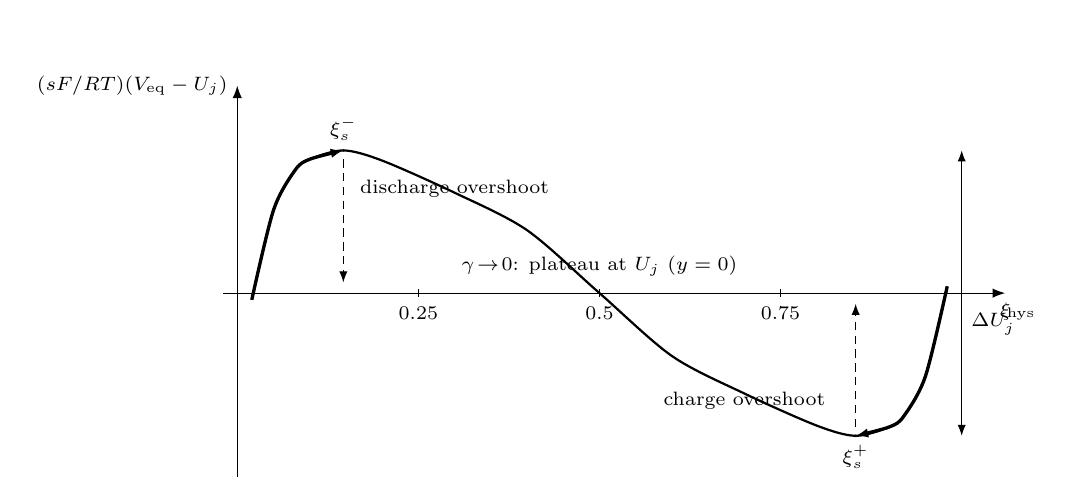
\begin{tikzpicture}[x=9.2cm,y=1.7cm]
\draw[-{Latex[length=1.6mm]}] (0,-1.45) -- (0,1.55) node[left,font=\scriptsize] {$(sF/RT)(V_\eq-U_j)$};
\draw[-{Latex[length=1.6mm]}] (-0.02,0) -- (1.06,0) node[below,font=\scriptsize] {$\xi$};
\foreach \xx in {0.25,0.5,0.75} {\draw (\xx,0.03) -- (\xx,-0.03) node[below,font=\scriptsize] {\xx};}
\draw[thick] plot[smooth] coordinates {(0.02,-0.05) (0.05,0.62) (0.08,0.92) (0.1,1.00) (0.1464,1.066) (0.2,0.99) (0.3,0.75) (0.4,0.47) (0.5,0) (0.6,-0.47) (0.7,-0.75) (0.8,-0.99) (0.8536,-1.066) (0.9,-1.00) (0.92,-0.92) (0.95,-0.62) (0.98,0.05)};
\fill (0.1464,1.066) circle (0.5pt) node[above,font=\scriptsize] {$\xi_s^-$};
\fill (0.8536,-1.066) circle (0.5pt) node[below,font=\scriptsize] {$\xi_s^+$};
\draw[{Latex[length=1.4mm]}-{Latex[length=1.4mm]}] (1.0,-1.066) -- (1.0,1.066) node[pos=0.4,right,font=\scriptsize] {$\Delta U_j^\hys$};
\draw[-{Latex[length=1.6mm]},very thick] plot[smooth] coordinates {(0.02,-0.05) (0.05,0.62) (0.08,0.92) (0.1,1.00) (0.1464,1.066)};
\draw[-{Latex[length=1.4mm]},densely dashed] (0.1464,1.0) -- (0.1464,0.08);
\node[font=\scriptsize] at (0.30,0.78) {discharge overshoot};
\draw[-{Latex[length=1.6mm]},very thick] plot[smooth] coordinates {(0.98,0.05) (0.95,-0.62) (0.92,-0.92) (0.9,-1.00) (0.8536,-1.066)};
\draw[-{Latex[length=1.4mm]},densely dashed] (0.8536,-1.0) -- (0.8536,-0.08);
\node[font=\scriptsize] at (0.70,-0.80) {charge overshoot};
\node[font=\scriptsize] at (0.5,0.20) {$\gamma\!\to\!0$: plateau at $U_j$ ($y=0$)};
\end{tikzpicture}
\caption{비단조 평형 전위 $V_\eq(\xi)$($\Omega_j=4RT$)와 과주행(v7-11). 방전(굵은 경로, 좌상)은 극대 $\xi_s^-$ 까지,
충전(우하)은 극소 $\xi_s^+$ 까지 과주행해 중심이 갈라진다. 두 극값 차가 spinodal 상한 gap $\Delta U_j^\hys$
(식~\eqref{eq:dUhys}), 실측 분기는 $\gamma_j$ 만큼 안쪽(식~\eqref{eq:Ubranch}).}
\label{fig:hysloop}
\end{figure}

% ====================================================================
\section{폭과 평형 점유 $\xi_\eq$ (N4, N5)}\label{sec:width}
% ====================================================================
중심이 정해지면 코드는 폭 $w_j$ 와 평형 점유 $\xi_{\eq,j}$ 를 평가한다.

\subsection{폭 $w_j$ — 이상 격자기체에서의 유도}

이상 격자기체($\Omega_j=0$)에서 화학퍼텐셜은 $\mu_{\mathrm{Li}}(\xi)=\mu^0+RT\ln[\xi/(1-\xi)]$ 다.
전기화학 평형 조건 $\mu_{\mathrm{Li}}(\xi_\eq)=\mu^0-sF(V-U_j)$ 를 대입하면 logit 형이 나오고, 그 등온선을 $V$ 로 미분할 때 나타나는 기울기 척도가 폭이다.

\begin{derivebox}
\textbf{출발.} $g_j'(\xi)=sF(V_\eq-U_j)$($\Omega=0$, 식~\eqref{eq:gxi} 로그 몫만):
\begin{equation*}
RT\ln\frac{\xi}{1-\xi}=sF(V-U_j).
\end{equation*}
\textbf{$\xi$ 로 미분.}
\begin{equation*}
\frac{RT}{\xi(1-\xi)}\cdot\frac{\dd\xi}{\dd V}=sF
\;\Longrightarrow\;
\frac{\dd\xi}{\dd V}=\frac{sF\,\xi(1-\xi)}{RT}.
\end{equation*}
\textbf{$z\equiv sF(V-U)/RT$ 로 환원.} $z$ 의 전위 기울기 $\dd z/\dd V=sF/RT=s/w$, $w\equiv RT/F$. 다중도 $n_j$ 로 일반화하면($w_j=n_jRT/F$):
\end{derivebox}
\begin{equation}
w_j=\frac{n_jRT}{F}\qquad(\text{기본 폭}),
\label{eq:wbase}
\end{equation}
코드 \code{func\_w(T, n)} 의 \code{n*R*T/F}. 상호작용이 종을 좁히는 유효 폭 옵션은
\begin{equation}
w_j^\eff=\frac{RT}{F}\Big(1-\frac{\Omega_j}{2RT}\Big),
\label{eq:weff}
\end{equation}
$\Omega_j\to2RT$ 에서 $0$ 으로 가므로 코드는 $\mathrm{floor\_frac}\cdot RT/F$ 하한으로 클립한다.

\subsection{평형 점유 $\xi_\eq$ — logistic 의 유도}

\begin{derivebox}
\textbf{출발: 정·역 속도와 detailed balance.}

정방향 속도(탈리튬화): $r^+=k_0\,e^{-(\Delta G_{a}-\chi\mathcal A)/RT}$ (빈 자리 $1-\xi$ 에서만 출발).

역방향 속도(재리튬화): $r^-=k_0\,e^{-(\Delta G_{a}+(1-\chi)\mathcal A)/RT}$ (찬 자리 $\xi$ 에서만 출발).

두 속도의 비:
\begin{equation*}
\frac{r^+}{r^-}=e^{\mathcal A/RT}\qquad(\text{detailed balance}).
\end{equation*}

\textbf{정지점 $\dd\xi/\dd t=0$ 설정.}
\begin{equation*}
r^+(1-\xi)=r^-\,\xi
\;\Longrightarrow\;
\frac{\xi}{1-\xi}=\frac{r^+}{r^-}=e^{\mathcal A/RT}.
\end{equation*}

\textbf{구동력 $\mathcal A=\sigma_d F(V-U_j^{\,d})$ 대입, $\xi$ 로 풀기.}
\begin{align*}
\frac{\xi}{1-\xi}&=e^{\sigma_d(V-U_j^{\,d})/w_j}\\
\xi\big(1+e^{-\sigma_d(V-U_j^{\,d})/w_j}\big)&=e^{\sigma_d(V-U_j^{\,d})/w_j}/(1+e^{\cdots})
\end{align*}
양변을 $(1+e^{-z})$, $z=\sigma_d(V-U_j^{\,d})/w_j$ 로 나누면:
\begin{equation*}
\xi_\eq=\frac{1}{1+e^{-z}}.
\end{equation*}
\end{derivebox}
\begin{equation}
\boxed{\;\xi_{\eq,j}(V,T)=\frac{1}{1+\exp\!\big[-\sigma_d(V-U_j^{\,d})/w_j\big]}\;.}
\label{eq:xieq}
\end{equation}
폭 다중도 $n_j$ 는 식~\eqref{eq:wbase} 의 $w_j=n_jRT/F$ 로 logistic 인자의 분모에 들어간다. 이것이
\code{func\_ksi\_eq(T, V\_n, U, n, s)} 의 $z=\sigma_d(V_\work-U_j^{\,d})/w_j$ 이며, 코드는 오버플로 방지를 위해
$z\ge0$ 과 $z<0$ 을 갈라 평가한다.

\begin{signbox}
\textbf{부호.} 방전 $\sigma_d=+1$: $V\!\uparrow\Rightarrow z\!\uparrow\Rightarrow\xi_\eq\!\uparrow$ — 전위를 올리면
탈리튬화 진행이 는다(규약 일치). 충전 $\sigma_d=-1$: $V\!\uparrow\Rightarrow z\!\downarrow\Rightarrow\xi_\eq\!\downarrow$.
극한 — $V=U_j^{\,d}\Rightarrow\xi_\eq=\tfrac12$(전이 중심). $w_j=RT/F=25.7$ mV($25^\circ$C).
\end{signbox}

\begin{figure}[t]
\centering
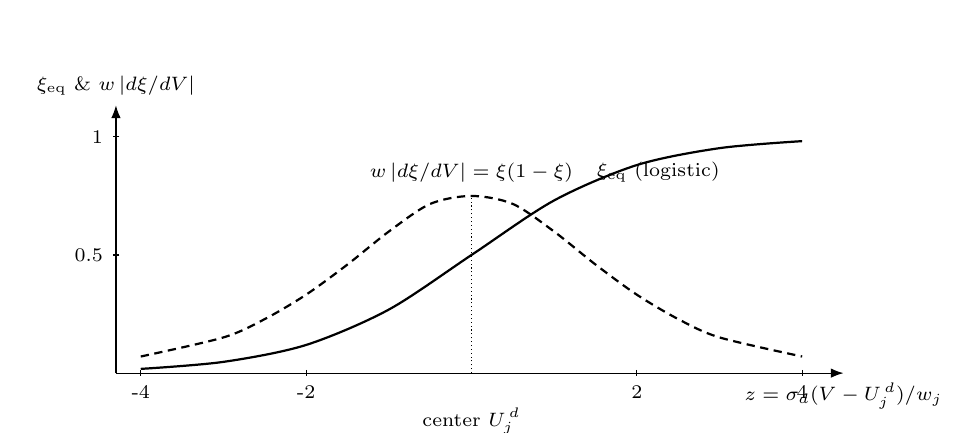
\begin{tikzpicture}[x=1.05cm,y=1.0cm]
\draw[-{Latex[length=1.6mm]}] (-4.3,0) -- (4.5,0) node[below,font=\scriptsize] {$z=\sigma_d(V-U_j^{\,d})/w_j$};
\draw[-{Latex[length=1.6mm]}] (-4.3,0) -- (-4.3,3.4) node[above,font=\scriptsize] {$\xi_\eq$ \&\ $w\,|d\xi/dV|$};
\foreach \xx in {-4,-2,2,4} {\draw (\xx,0.04) -- (\xx,-0.04) node[below,font=\scriptsize] {\xx};}
\draw (-4.26,3.0) -- (-4.34,3.0) node[left,font=\scriptsize] {1};
\draw (-4.26,1.5) -- (-4.34,1.5) node[left,font=\scriptsize] {0.5};
% xi_eq scaled by 3
\draw[thick] plot[smooth] coordinates {(-4,0.0537) (-3,0.1429) (-2,0.3577) (-1,0.8068) (0,1.5) (1,2.1932) (2,2.6423) (3,2.8571) (4,2.9463)};
\node[right,font=\scriptsize] at (1.4,2.55) {$\xi_\eq$ (logistic)};
% derivative xi(1-xi) max 0.25 scaled by 12 -> max 3
\draw[densely dashed,thick] plot[smooth] coordinates {(-4,0.211) (-3,0.4534) (-2.5,0.6864) (-2,0.9963) (-1.5,1.3792) (-1,1.7976) (-0.5,2.1487) (0,2.25) (0.5,2.1487) (1,1.7976) (1.5,1.3792) (2,0.9963) (2.5,0.6864) (3,0.4534) (4,0.211)};
\node[font=\scriptsize] at (0,2.55) {$w\,|d\xi/dV|=\xi(1-\xi)$};
\draw[densely dotted] (0,0)--(0,2.25);
\node[below,font=\scriptsize] at (0,-0.32) {center $U_j^{\,d}$};
\end{tikzpicture}
\caption{평형 점유와 그 미분(v7-11). 실선 $=\xi_\eq$ logistic(식~\eqref{eq:xieq}), 파선 $=$ 폭으로 규격화한 미분
$w_j|d\xi_\eq/dV|=\xi_\eq(1-\xi_\eq)$ — $z=0$(중심 $U_j^{\,d}$)에서 최대 $\tfrac14$ 인 종 모양. 이 종이
다음 절의 평형 peak 이고, 방향에 불변(양수)이다.}
\label{fig:logistic}
\end{figure}

% ====================================================================
\section{평형 peak — $|I|\to0$ 기준선 (N6)}\label{sec:eqpeak}
% ====================================================================
코드는 평형 점유에서 곧바로 평형 peak 모양 $\xi_\eq(1-\xi_\eq)/w$ 를 만든다.

\subsection{관측 $\dd Q/\dd V$ 의 전하 보존식 유도}

전하 보존식 $Q_\cell q=Q_\bg(V_n)+\sum_jQ_j\xi_j$ 를 궤적 $q$ 로 미분하면

\begin{derivebox}
\textbf{출발.} 양변을 $q$ 로 미분:
\begin{equation*}
Q_\cell=C_\bg\,\frac{\dd V_n}{\dd q}+\sum_j Q_j\,\frac{\dd\xi_j}{\dd q}.
\end{equation*}
\textbf{$\dd V_n/\dd q$ 로 나누기(연쇄율):}
\begin{equation*}
\frac{\dd Q}{\dd V_n}=\frac{Q_\cell}{\dd V_n/\dd q}=C_\bg+\sum_j Q_j\frac{\dd\xi_j}{\dd V_n}.
\end{equation*}
\textbf{평형 추종 대입.} $\dd\xi_j/\dd V_n$ 에 평형 기울기를 넣는다. $z=\sigma_d(V-U_j^{\,d})/w_j$ 로 치환하면
$\xi_\eq=(1+e^{-z})^{-1}$ 이고
\begin{equation*}
\frac{\dd\xi_\eq}{\dd z}
=\frac{e^{-z}}{(1+e^{-z})^2}
=\underbrace{\frac{1}{1+e^{-z}}}_{\xi_\eq}\cdot\underbrace{\frac{e^{-z}}{1+e^{-z}}}_{1-\xi_\eq}
=\xi_\eq(1-\xi_\eq).
\end{equation*}
연쇄율 $\dd z/\dd V=\sigma_d/w_j$ 를 곱하면 $\dd\xi_\eq/\dd V=\sigma_d\xi_\eq(1-\xi_\eq)/w_j$.
peak 모양은 절댓값 $|\dd\xi/\dd V|=\xi_\eq(1-\xi_\eq)/w_j$, 방향 불변.
\end{derivebox}
\begin{equation}
\frac{\dd\xi_{\eq,j}}{\dd V}=\frac{\sigma_d\,\xi_{\eq,j}(1-\xi_{\eq,j})}{w_j}
\;\Longrightarrow\;
\boxed{\;\Big(\frac{\dd Q}{\dd V}\Big)^\eq_j
=Q_j\,\frac{\xi_{\eq,j}(1-\xi_{\eq,j})}{w_j}\;.}
\label{eq:eqpeak}
\end{equation}
이것이 코드의 \code{peak\_shape = ksi\_eq * (1 - ksi\_eq) / w} 이며, 메서드 \code{equilibrium} 이 전이별로 이 항만
합산한다. 부호 — peak 모양 $=|\dd\xi/\dd V|=\xi_\eq(1-\xi_\eq)/w\ge0$, 방향 불변. 세 양 — 위치 $=$ 중심
$U_j^{\,d}$, 순높이 $=Q_j/(4w_j)$($\xi=\tfrac12$ 에서 $\xi(1-\xi)=\tfrac14$), 면적 $=Q_j$ — 가 이 한 식에서 읽힌다.

% ====================================================================
\section{동역학 지연 길이 $L_V$ (N7)}\label{sec:lag}
% ====================================================================
유한 전류에서는 평형 목표 $\xi_\eq$ 를 점유가 즉시 따라가지 못하고 뒤처진다 — 그 지연이 peak 의 꼬리다.
이 절은 사슬 $\mathcal A\to\chi_d\to\Delta H_a^\eff\to L_q\to L_V$ 를 닫는다.

\subsection{보편 지연 방정식과 용량축 길이 $L_q$ 의 유도}

\begin{derivebox}
\textbf{출발.} 운동방정식 $\dd\xi_j/\dd t=k_j(\xi_{\eq,j}-\xi_j)$, 정전류 $\dd q/\dd t=|I|/Q_\cell$.

\textbf{$t$ 대신 $q$ 로 기술.} 양변을 $\dd q/\dd t$ 로 나누면
\begin{equation*}
\frac{\dd\xi_j}{\dd q}=\frac{Q_\cell\,k_j}{|I|}\,(\xi_{\eq,j}-\xi_j).
\end{equation*}

\textbf{지연 $r_j\equiv\xi_{\eq,j}-\xi_j$ 의 방정식.} $\dd r_j/\dd q=\dd\xi_{\eq,j}/\dd q-\dd\xi_j/\dd q$ 에 위 식을 대입:
\begin{equation*}
\frac{\dd r_j}{\dd q}=\frac{\dd\xi_{\eq,j}}{\dd q}-\frac{Q_\cell k_j}{|I|}(\xi_{\eq,j}-\xi_j)
=\frac{\dd\xi_{\eq,j}}{\dd q}-\frac{r_j}{L_{q,j}},
\qquad L_{q,j}\equiv\frac{|I|}{Q_\cell k_j}.
\end{equation*}
\end{derivebox}
\begin{equation}
\frac{\dd r_j}{\dd q}=\frac{\dd\xi_{\eq,j}}{\dd q}-\frac{r_j}{L_{q,j}},
\qquad L_{q,j}=\frac{|I|}{Q_\cell\,k_j}.
\label{eq:Lq}
\end{equation}
$L_{q,j}$ 는 요구($|I|/Q_\cell$)와 공급($k_j$) 의 비 그 자체다. 완화 속도 $k_j$ 는 정$\cdot$역 속도의 합이다:
\begin{equation}
k_j=r_j^++r_j^-=r_j^+\big(1+e^{-\mathcal A_j/RT}\big)\qquad(\text{detailed balance: }r_j^-=r_j^+e^{-\mathcal A_j/RT}).
\label{eq:kuniv}
\end{equation}

\subsection{컷 affinity $\mathcal A$ — 꼬리 시작점의 구동력}

$L_q$ 는 전이당 한 점(꼬리 컷점 $q_a$)에서 \emph{상수로 동결}된다. 원천 $\dd\xi_\eq/\dd q$ 가 정점의 $5\%$ 로 떨어지는
좌표에서 구동력이 $\mathcal A=z_\mathrm{cut}\cdot n_jRT$($z_\mathrm{cut}=4.357$)이고, 상한과 함께
\begin{equation}
\mathcal A=\min\!\big(z_\mathrm{cut}\,n_j\,RT,\;A_\mathrm{cap}\,RT\big),
\qquad z_\mathrm{cut}=4.357,\ A_\mathrm{cap}=4.0\ (\text{기본}).
\label{eq:Acut}
\end{equation}
\emph{부호의 핵심} — 컷 affinity 의 \emph{크기}는 충$\cdot$방전 동일($n_j>0$ 라 항상 양수)이고, 방향은 아래 $\chi_d\cdot\Delta H_a^\eff$ 가 받는다.

\subsection{방향별 전달 계수와 유효 장벽의 유도}

\begin{derivebox}
\textbf{출발.} 정$\cdot$역 속도(식~\eqref{eq:kuniv} 계열):
\begin{equation*}
r_j^+=k_0\,e^{-(\Delta G_{a,j}-\chi\mathcal A_j)/RT},\quad
r_j^-=k_0\,e^{-(\Delta G_{a,j}+(1-\chi)\mathcal A_j)/RT}.
\end{equation*}

\textbf{합-1 제약(detailed balance).}
\begin{equation*}
\frac{r_j^+}{r_j^-}=e^{\mathcal A_j/RT}\;\overset{!}{=}\;e^{\mathcal A_j/RT}
\;\Longrightarrow\;\chi+(1-\chi)=1\quad(\forall\mathcal A_j).
\end{equation*}
방전은 $\xi\to1$ 깊은 꼬리에서 역방향 장벽의 상수 몫 $+\Omega$ 가 흡수되고,
충전은 거울이라 $1-\chi$ 가 받는다.
\end{derivebox}
\begin{equation}
\chi_d=\chi_\mathrm{split}(\chi,\sigma_d)=
\begin{cases}\chi & \sigma_d\ge0\ (\text{방전})\\ 1-\chi & \sigma_d<0\ (\text{충전}).\end{cases}
\label{eq:chid}
\end{equation}
\begin{equation}
\boxed{\;\Delta H_{a,j}^\eff=\Delta H_{a,j}-\chi_d\,\Omega_j\;.}
\label{eq:dHeff}
\end{equation}
이것이 \code{func\_dH\_a\_eff(dH\_a, Omega, chi\_d)} 이다.

\subsection{$L_q$ 의 평가와 전압축 환산 $L_V$ 의 유도}

\begin{derivebox}
\textbf{출발.} 식~\eqref{eq:kuniv} 의 $k_j=r_j^+(1+e^{-\mathcal A/RT})$, Eyring: $r_j^+=k_0\,e^{-(\Delta G_{a,j}^\eff-\chi_d\mathcal A)/RT}$,
$k_0=k_BT/h$.

\textbf{$k_j$ 전개.}
\begin{equation*}
k_j=\frac{k_BT}{h}\,e^{-(\Delta H_{a,j}^\eff-T\Delta S_{a,j}-\chi_d\mathcal A)/RT}\,(1+e^{-\mathcal A/RT}).
\end{equation*}

\textbf{$L_{q,j}=|I|/(Q_\cell k_j)$ 대입.} $T_*\equiv|I|h/(Q_\cell k_B)$ 로 정의:
\begin{align*}
L_{q,j}&=\frac{|I|}{Q_\cell}\cdot\frac{h}{k_BT}\cdot
\frac{e^{(\Delta H_{a,j}^\eff-T\Delta S_{a,j}-\chi_d\mathcal A)/RT}}{1+e^{-\mathcal A/RT}}
\cdot e^{0}\cdot e^{\chi_d\mathcal A/RT}\cdot e^{-\chi_d\mathcal A/RT}\\
&=\frac{T_*}{T}\cdot
\frac{e^{(\Delta H_{a,j}^\eff-T\Delta S_{a,j})/RT}}{1+e^{-\mathcal A/RT}}
\cdot e^{-\chi_d\mathcal A/RT}.
\end{align*}
로그 4항 분해:
$\ln L_q=\ln(T_*/T)-\ln(1+e^{-\mathcal A/RT})+(\Delta H_{a,j}^\eff-T\Delta S_{a,j})/(RT)-\chi_d\mathcal A/(RT)$.
\end{derivebox}
\begin{equation}
L_{q,j}=\frac{T_*}{T}\,\frac{\exp\!\big[(\Delta H_{a,j}^\eff-T\Delta S_{a,j})/RT\big]}{1+e^{-\mathcal A/RT}}
\,e^{-\chi_d\mathcal A/RT},
\qquad T_*\equiv\frac{|I|\,h}{Q_\cell\,k_B}.
\label{eq:Lqfull}
\end{equation}
코드의 \code{func\_L\_q} 가 이 로그 4항을 합산해 지수화한다. 전압축 환산은 컷점 OCV 기울기를 곱한다:
\begin{equation}
\boxed{\;L_{V,j}=\Big|\frac{\dd V}{\dd q}\Big|_{q_a}\,L_{q,j}\;=\;|\code{dVdq\_qa}|\cdot L_{q,j}\;.}
\label{eq:LV}
\end{equation}

\emph{부호의 핵심} — 컷 affinity $\mathcal A$ 가 전이당 컷 상수라, 코드 안에서 $L_q$ 는 $V$ 의 함수로 다시 미분되지
않는다: \emph{운영상 실현 미분은} $\partial\ln L_q/\partial V=0$(전이당 한 스칼라). 부등식 $\partial\ln L_q/\partial V<0$ 은
\emph{물리적 동기}로 읽어야 한다 — 국소 구동력으로 두면 $V\!\uparrow\Rightarrow\mathcal A\!\uparrow\Rightarrow$
유효 장벽$\downarrow\Rightarrow L_q\downarrow$(꼬리 짧아짐)이 되어, 이 단조성이 컷 규칙의 정당성이다. 그러나 코드는
컷 상수를 쓰므로 운영상 미분은 $0$ 이다. 한편 $|I|$ 의존은 동결 뒤에도 살아 있다 — $L_q\propto|I|$($T_*\propto|I|$)라
$|I|\to0$ 에서 $L_V\to0$ 이고 다음 절의 꼬리가 사라져 평형 peak 으로 환원된다.

\begin{figure}[t]
\centering
% L_q chain diagram (new)
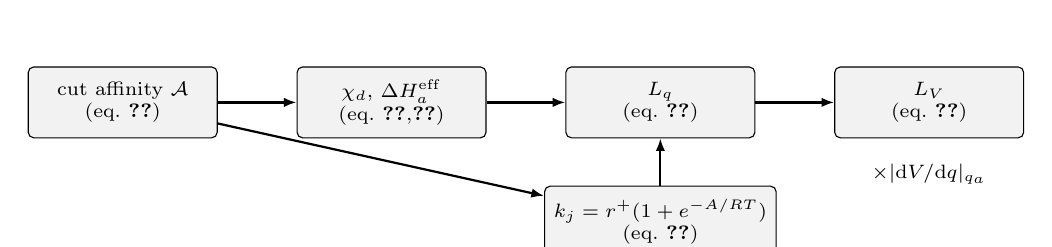
\begin{tikzpicture}[
  box/.style={draw,rounded corners=2pt,minimum width=2.4cm,minimum height=0.9cm,align=center,font=\scriptsize,fill=black!5},
  ar/.style={-{Latex[length=1.6mm]},thick},
  node distance=6mm and 10mm]
\node[box] (A) {cut affinity $\mathcal A$\\(eq.~\ref{eq:Acut})};
\node[box,right=of A] (C) {$\chi_d$, $\Delta H_a^\eff$\\(eq.~\ref{eq:chid},\ref{eq:dHeff})};
\node[box,right=of C] (L) {$L_q$\\(eq.~\ref{eq:Lqfull})};
\node[box,right=of L] (LV) {$L_V$\\(eq.~\ref{eq:LV})};
\node[box,below=of L] (k) {$k_j = r^+(1+e^{-A/RT})$\\(eq.~\ref{eq:kuniv})};
\draw[ar] (A) -- (C);
\draw[ar] (C) -- (L);
\draw[ar] (L) -- (LV);
\draw[ar] (A) -- (k);
\draw[ar] (k) -- (L);
\node[font=\scriptsize,below=2mm of LV] {$\times|\dd V/\dd q|_{q_a}$};
\end{tikzpicture}
\caption{$L_q\to L_V$ 사슬 개요(신규). 컷 affinity $\mathcal A$ 에서 $(\chi_d, \Delta H_a^\eff)$ 를 거쳐 용량축 길이
$L_q$, 컷점 OCV 기울기로 전압축 길이 $L_V$ 까지의 단방향 의존 사슬. 각 화살표에 해당 식 번호를 달았다.}
\label{fig:lq_chain}
\end{figure}

\begin{codebox}
\textbf{N7 진행.} \code{n\_safe=|n\_j|} $\to$ $\mathcal A$(식~\eqref{eq:Acut}) $\to$
\code{(chi\_d, dH\_a\_use)=\_chi\_and\_dH\_eff(...)} (식~\eqref{eq:chid}$\cdot$\eqref{eq:dHeff}) $\to$
\code{L\_q=func\_L\_q(...,x=chi\_d,A=A)} (식~\eqref{eq:Lqfull}) $\to$ \code{L\_V=|dVdq\_qa|*L\_q} (식~\eqref{eq:LV}).
전이당 \emph{상수}(대표 $T_\rep$)로 한 번 평가한다.
\end{codebox}

% ====================================================================
\section{인과 기억 꼬리와 충전 격자 역전 (N8)}\label{sec:tail}
% ====================================================================
지연 길이 $L_{V,j}$ 가 충분히 크면 코드는 평형 종 대신 \emph{인과 기억 꼬리}를 만든다.

\subsection{지수 기억 — 일반해의 이산형 유도}

\begin{derivebox}
\textbf{출발.} 식~\eqref{eq:Lq} 는 1계 선형 ODE다. 적분인자 $e^{q/L_{q,j}}$ 를 곱하면:
\begin{equation*}
\frac{\dd}{\dd q}\Big(r_j\,e^{q/L_{q,j}}\Big)
=e^{q/L_{q,j}}\Big(\frac{\dd r_j}{\dd q}+\frac{r_j}{L_{q,j}}\Big)
=e^{q/L_{q,j}}\,\frac{\dd\xi_{\eq,j}}{\dd q}.
\end{equation*}

\textbf{$q_0$부터 $q$까지 적분.} 좌변은 양 끝값의 차:
\begin{equation*}
r_j(q)\,e^{q/L_q}-r_j(q_0)\,e^{q_0/L_q}
=\int_{q_0}^q e^{q'/L_q}\,\frac{\dd\xi_{\eq,j}}{\dd q'}\,\dd q'.
\end{equation*}

\textbf{$e^{-q/L_q}$ 곱해 $r_j(q)$ 정리.}
\begin{equation*}
r_j(q)=r_j(q_0)\,e^{-(q-q_0)/L_q}
+\int_{q_0}^q e^{-(q-q')/L_q}\,\frac{\dd\xi_{\eq,j}}{\dd q'}\,\dd q'.
\end{equation*}

\textbf{이산 격자 근사.} 한 칸 $\Delta_\mathrm{grid}$ 에서 지수 커널을 감쇠 $\rho=e^{-\Delta_\mathrm{grid}/L_V}$ 로 근사하면 점화식:
\begin{equation*}
\xi_{\mathrm{lag},i}=\rho\,\xi_{\mathrm{lag},i-1}+(1-\rho)\,\xi_{\eq,i}.
\end{equation*}
\end{derivebox}
\begin{equation}
\xi_{\mathrm{lag},i}=\rho\,\xi_{\mathrm{lag},i-1}+(1-\rho)\,\xi_{\eq,i},
\qquad\rho=\exp(-\Delta_\mathrm{grid}/L_V).
\label{eq:lowpass}
\end{equation}
코드 \code{\_causal\_lowpass} 가 이를 \code{scipy.signal.lfilter} 의 계수 $[1-\rho]/[1,-\rho]$ 로 평가한다.

\subsection{peak 모양 — 평형에서 지연을 뺀 것}

꼬리를 포함한 peak 모양은 ``평형 점유에서 지연된 점유를 뺀 것을 길이로 나눈'' 이산 미분이다:
\begin{equation}
\boxed{\;\text{peak\_shape}=\frac{\xi_{\eq}-\xi_{\mathrm{lag}}}{L_{V,j}}\;.}
\label{eq:peakshape}
\end{equation}
$L_V$ 가 작으면 $\xi_\mathrm{lag}\to$ 한 칸 뒤처진 $\xi_\eq$ 라, 식~\eqref{eq:peakshape} 가 이산 미분
$\to\dd\xi_\eq/\dd V$ 의 종으로 환원된다 — 평형 peak 식~\eqref{eq:eqpeak} 로 돌아간다.
\begin{equation}
\text{peak\_shape}=
\begin{cases}
\xi_\eq(1-\xi_\eq)/w & L_{V,j}<\nu\,\Delta_\mathrm{grid}\quad[\text{평형, 식~\eqref{eq:eqpeak}}]\\[2pt]
(\xi_\eq-\xi_\mathrm{lag})/L_{V,j} & \text{그 외}\quad[\text{꼬리, 식~\eqref{eq:peakshape}}],
\end{cases}
\label{eq:branch}
\end{equation}
$\nu=\code{min\_lag\_grid\_steps}=2$ 다.

\subsection{★충전 격자 역전 — 인과 방향}

인과 합성곱은 ``진행 방향의 과거''를 기억한다. 방전($\sigma_d=+1$)은 진행이 $V$ 증가 방향이라 격자 그대로 적용한다. 충전($\sigma_d=-1$)은 진행이 $V$ 감소 방향 — 격자 오름차순의 \emph{역}이 시간 순서이므로, 충전은 격자를 뒤집어 필터하고 되돌린다:
\begin{equation}
\xi_\mathrm{lag}=
\begin{cases}
\code{causal\_lowpass}(\xi_\eq) & \sigma_d\ge0\ (\text{방전})\\[2pt]
\code{causal\_lowpass}(\xi_\eq[::-1])[::-1] & \sigma_d<0\ (\text{충전}).
\end{cases}
\label{eq:reversal}
\end{equation}
이 역전이 없으면 충전 꼬리가 미래를 기억하는 비인과 신호가 된다. \emph{부호 결과} — 충전 $\dd Q/\dd V$ 는 방전의
거울상이고, peak\_shape $=(\xi_\eq-\xi_\mathrm{lag})/L_V$ 는 양수를 유지한다.

\begin{figure}[t]
\centering
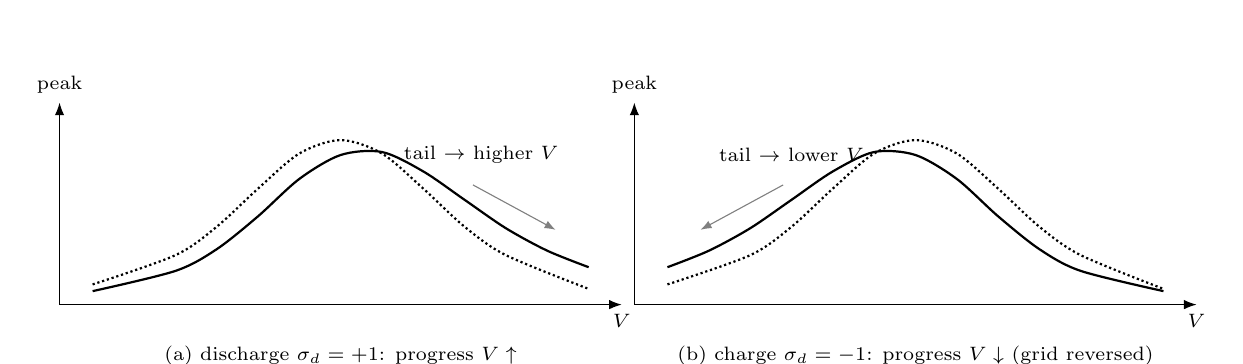
\begin{tikzpicture}[x=1.05cm,y=0.95cm]
\begin{scope}
\draw[-{Latex[length=1.6mm]}] (-3.4,0) -- (3.4,0) node[below,font=\scriptsize] {$V$};
\draw[-{Latex[length=1.6mm]}] (-3.4,0) -- (-3.4,2.7) node[above,font=\scriptsize] {peak};
\draw[densely dotted,thick] plot[smooth] coordinates {(-3,0.27) (-2,0.66) (-1.5,1.04) (-1,1.55) (-0.5,2.02) (0,2.2) (0.5,2.02) (1,1.55) (1.5,1.04) (2,0.66) (3,0.21)};
\draw[thick] plot[smooth] coordinates {(-3,0.18) (-2,0.45) (-1.5,0.74) (-1,1.18) (-0.5,1.68) (0,2.0) (0.5,2.04) (1,1.78) (1.5,1.4) (2,1.02) (2.5,0.72) (3,0.5)};
\draw[-{Latex[length=1.4mm]},gray] (1.6,1.6)--(2.6,1.0);
\node[font=\scriptsize] at (1.7,2.0) {tail $\to$ higher $V$};
\node[font=\scriptsize,below] at (0,-0.42) {(a) discharge $\sigma_d=+1$: progress $V\uparrow$};
\end{scope}
\begin{scope}[xshift=7.3cm]
\draw[-{Latex[length=1.6mm]}] (-3.4,0) -- (3.4,0) node[below,font=\scriptsize] {$V$};
\draw[-{Latex[length=1.6mm]}] (-3.4,0) -- (-3.4,2.7) node[above,font=\scriptsize] {peak};
\draw[densely dotted,thick] plot[smooth] coordinates {(-3,0.27) (-2,0.66) (-1.5,1.04) (-1,1.55) (-0.5,2.02) (0,2.2) (0.5,2.02) (1,1.55) (1.5,1.04) (2,0.66) (3,0.21)};
\draw[thick] plot[smooth] coordinates {(-3,0.5) (-2.5,0.72) (-2,1.02) (-1.5,1.4) (-1,1.78) (-0.5,2.04) (0,2.0) (0.5,1.68) (1,1.18) (1.5,0.74) (2,0.45) (3,0.18)};
\draw[-{Latex[length=1.4mm]},gray] (-1.6,1.6)--(-2.6,1.0);
\node[font=\scriptsize] at (-1.5,2.0) {tail $\to$ lower $V$};
\node[font=\scriptsize,below] at (0,-0.42) {(b) charge $\sigma_d=-1$: progress $V\downarrow$ (grid reversed)};
\end{scope}
\end{tikzpicture}
\caption{인과 꼬리의 방향(v7-11). 점선 $=$ 평형 종($\xi_\eq(1-\xi_\eq)/w$, 방향 불변). 실선 $=$ peak\_shape with tail.
(a) 방전은 꼬리가 높은 $V$ 쪽으로 늘어진다(격자 그대로). (b) 충전은 격자를 뒤집어 필터($\xi[::-1]\cdots[::-1]$)해 꼬리가 낮은 $V$ 쪽으로 — 방전의 거울. 두 경우 모두 peak 는 양수.}
\label{fig:reversal}
\end{figure}

% ====================================================================
\section{합산과 역보간 (N9)}\label{sec:sum}
% ====================================================================
전이 루프가 각 전이의 peak\_shape 를 (식~\eqref{eq:branch} 의 두 분기로) 만들면, 코드는 용량 가중을 곱해 작업 격자 위
누적에 더하고, 모든 전이가 끝나면 내부 전위 격자로 역보간한다. 보존식 $Q_\cell q=Q_\bg+\sum_jQ_j\xi_j$ 의 선형 구조에서
관측 ICA 는 배경과 전이별 기여의 선형 합이다:
\begin{equation}
\boxed{\;\frac{\dd Q}{\dd V}(V_n)\;=\;C_\bg\;+\;\sum_{j=1}^{N_p}Q_j\,
\big[\text{peak\_shape}_j\big]
\;=\;C_\bg+\sum_jQ_j\big[\text{평형 peak}-\text{지연 꼬리}\big]\;.}
\label{eq:sum}
\end{equation}
코드는 \code{dqdv\_work += tr['Q'] * peak\_shape} 로 누적하고(배경은 루프 전에 깔림), 마지막에
\code{np.interp(V\_n, V\_work, dqdv\_work)} 로 역보간한다.

\subsection{staging 전이 초기값 — 피팅 출발점}

\begin{table}[t]
\centering
\renewcommand{\arraystretch}{1.25}
\caption{전이 초기값 \code{GRAPHITE\_STAGING\_LIT}(4건) — 출발점, 피팅으로 override. $U$ 는 \code{'U'}
폴백이자 $(\Delta H_\rxn,\Delta S_\rxn)$ 정합 목표.}
\label{tab:staging}
\begin{tabular}{l c c c c c c c}
\toprule
stage & $U$ [V] & $\Delta H_\rxn$ & $\Delta S_\rxn$ & $Q$ & $\Omega$ & $\Delta H_a$ & $|\dd V/\dd q|_{q_a}$ \\
 &  & [J/mol] & [J/(mol\,K)] & [$Q_\cell$] & [J/mol] & [J/mol] & [V] \\
\midrule
$4\!\to\!3$   & 0.210 & $-11700$ & $+29.0$ & 0.10 & 6000  & 48000 & 0.30 \\
$3\!\to\!2\mathrm L$ & 0.140 & $-13500$ & $0.0$   & 0.12 & 8000  & 46000 & 0.30 \\
$2\mathrm L\!\to\!2$ & 0.120 & $-13100$ & $-5.0$  & 0.25 & 10000 & 44000 & 0.30 \\
$2\!\to\!1$   & 0.085 & $-13000$ & $-16.0$ & 0.50 & 13000 & 40000 & 0.30 \\
\bottomrule
\end{tabular}
\end{table}

\subsection{전체 입력 인자와 기본값 — 피팅 준비}

\begin{table}[t]
\centering\footnotesize
\renewcommand{\arraystretch}{1.18}
\caption{전체 입력 인자(코드 식별자)와 기본값.}
\label{tab:inputs}
\begin{tabular}{l l l l}
\toprule
인자(코드) & 자리 & 기본값 & 곡선 내 역할(식) \\
\midrule
\multicolumn{4}{l}{\emph{— 전이 dict 키(전이별) —}}\\
\code{U} 또는 (\code{dH\_rxn},\code{dS\_rxn}) & 전이 & --- & 평형 중심 $U_j(T)$ (\eqref{eq:Uj}) \\
\code{w} 또는 \code{n} & 전이 & --- / $1$ & 폭 $w_j=n_jRT/F$ (\eqref{eq:wbase}) \\
\code{Q} & 전이 & --- & 용량 가중(면적) \\
\code{Omega},\code{gamma} & 전이 & $0$,\,$0$ & 상호작용$\cdot$분기(히스, \eqref{eq:dUhys}\eqref{eq:Ubranch}) \\
\code{h\_eta} & 전이 & $1.0$ & 부분 cycle 분기 인자 \\
\code{dH\_a},\code{dS\_a} & 전이 & --- / $0$ & 활성화(꼬리, \eqref{eq:Lqfull}) \\
\code{dVdq\_qa} & 전이 & $0$ & 컷 OCV 기울기 $L_q\!\to\!L_V$ (\eqref{eq:LV}) \\
\code{L\_V} & 전이 & --- & 직접 지연 길이(동역학 우회) \\
\code{z\_cut},\code{A\_cap\_RT} & 전이/공통 & $4.357$,\,$4.0$ & 컷 affinity (\eqref{eq:Acut}) \\
\code{use\_w\_eff},\code{use\_dH\_eff} & 전이/공통 & False,\,True & 옵션 토글(\eqref{eq:weff},\eqref{eq:dHeff}) \\
\multicolumn{4}{l}{\emph{— 생성자 인자(모델 공통) —}}\\
\code{x}/\code{chi},\,\code{chi\_split} & 공통 & $0.5$,\,\code{func\_chi\_d} & 전달 계수 $\chi_d$ (\eqref{eq:chid}) \\
\code{Rn} & 공통 & $0.0$ & 분극 저항 (\eqref{eq:vn}) \\
\code{Cbg} & 공통 & $0.0$ & 배경 $C_\bg$ \\
\code{grid\_pad\_lo/hi},\,\code{n\_work\_min} & 공통 & $0.15$,\,$2048$ & 작업 격자 (\eqref{eq:vwork}) \\
\code{min\_lag\_grid\_steps} & 공통 & $2.0$ & 꼬리/평형 전환 문턱 (\eqref{eq:branch}) \\
\bottomrule
\end{tabular}
\end{table}

\begin{keybox}
\textbf{이 문건만으로 한 곡선 재현(6단계).}
(1) 표~\ref{tab:staging} 의 4 전이로 \code{transitions} 구성.
(2) $\sigma_d$, $|I|$, $T$, $R_n$ 설정 → $V_n$(\eqref{eq:vn}), $V_\work$(\eqref{eq:vwork}).
(3) 전이마다 $U_j(T)$(\eqref{eq:Uj}) → 분기 중심(\eqref{eq:center}) → $w_j$(\eqref{eq:wbase}) → $\xi_\eq$(\eqref{eq:xieq}).
(4) $\mathcal A$(\eqref{eq:Acut}) → $\chi_d,\Delta H_a^\eff$(\eqref{eq:chid}\eqref{eq:dHeff}) → $L_q$(\eqref{eq:Lqfull}) → $L_V$(\eqref{eq:LV}).
(5) peak\_shape: $L_V<2\Delta_\mathrm{grid}$ 면 평형 종(\eqref{eq:eqpeak}), 아니면 인과 꼬리(\eqref{eq:peakshape}, 충전 격자 역전 \eqref{eq:reversal}).
(6) 용량 가중 합산 후 $V_n$ 으로 역보간(\eqref{eq:sum}).
\end{keybox}

\begin{table}[t]
\centering
\renewcommand{\arraystretch}{1.3}
\caption{노드 $\leftrightarrow$ 식 $\leftrightarrow$ 코드 식별자 매핑(전체 진행).}
\label{tab:nodemap}
\begin{tabular}{l l l l}
\toprule
노드 & 물리식 & 본 문건 식 & 코드 식별자 \\
\midrule
N0 & $\sigma_d,|I|=\code{c\_rate}\,Q_\cell$ & \eqref{eq:n0map} & \code{curve},\code{\_direction\_to\_sigma} \\
N1 & $V_n=V_\app-\sigma_d|I|R_n$ & \eqref{eq:vn} & \code{dqdv} L412 \\
N2 & $U_j(T)=(-\Delta H+T\Delta S)/F$ & \eqref{eq:Uj} & \code{func\_U\_j} \\
N3 & $\Delta U_j^\hys$, $U_j^{\,d}$ & \eqref{eq:dUhys},\eqref{eq:Ubranch} & \code{func\_dU\_hys},\code{func\_U\_branch} \\
N4 & $w_j=n_jRT/F$ ($w^\eff$) & \eqref{eq:wbase}(\eqref{eq:weff}) & \code{func\_w},\code{func\_w\_eff} \\
N5 & $\xi_\eq=\mathrm{logistic}[\sigma_d(V-U^d)/w]$ & \eqref{eq:xieq} & \code{func\_ksi\_eq} \\
N6 & $Q_j\xi_\eq(1-\xi_\eq)/w$ & \eqref{eq:eqpeak} & \code{equilibrium}, 인라인 \\
N7 & $\mathcal A,\chi_d,\Delta H_a^\eff,L_q,L_V$ & \eqref{eq:Acut}--\eqref{eq:LV} & \code{\_resolve\_lag\_length},\code{func\_L\_q} \\
N8 & $(\xi_\eq-\xi_\mathrm{lag})/L_V$, 역전 & \eqref{eq:peakshape},\eqref{eq:reversal} & \code{\_causal\_lowpass} \\
N9 & $C_\bg+\sum_jQ_j[\cdot]$ & \eqref{eq:sum} & \code{dqdv\_work},\code{np.interp} \\
\bottomrule
\end{tabular}
\end{table}

% ====================================================================
\section{부호 사슬 전수 검산}\label{sec:signcheck}
% ====================================================================
브리프 §7 의 부호 체크리스트를 전건 확인한다 — 한 곳이라도 어긋나면 결함이다. 기준 명제 = \emph{방전 시
$V\!\uparrow\Rightarrow$ 탈리튬화$\uparrow$, 충전 $\dd Q/\dd V$ 는 방전의 거울(양수)}.

\begin{enumerate}[label=\textbf{S\arabic*.},leftmargin=2.6em,itemsep=2pt]
\item \textbf{$U_j(T)=(-\Delta H+T\Delta S)/F$, $\Delta G=-FU$.} 식~\eqref{eq:Uj}$\cdot$\eqref{eq:eqcond}. $\Delta H_\rxn<0$
(발열)이면 $-\Delta H_\rxn>0$ 이 중심을 올린다. $\Delta G_j=-sFU_j$ 부호 일치. $\checkmark$
\item \textbf{$\xi_\eq=\mathrm{logistic}[\sigma_d(V-U)/w]$.} 식~\eqref{eq:xieq}. 방전 $\sigma_d=+1$ 에서
$V\!\uparrow\Rightarrow\xi_\eq\!\uparrow$. $\checkmark$
\item \textbf{$d\xi/dV=\sigma_d\,\xi(1-\xi)/w$, peak 양수.} 식~\eqref{eq:eqpeak}. peak 모양 $=|\dd\xi/\dd V|=
\xi(1-\xi)/w\ge0$, 방향 불변. $\checkmark$
\item \textbf{$\Delta U_\hys\ge0$, $\Omega\le2RT\to0$; 분기 중심 $\pm\tfrac12\sigma_d$.} 식~\eqref{eq:dUhys}$\cdot$
\eqref{eq:Ubranch}. 극대 $>$ 극소라 $\ge0$; $u_j\to0$ 에서 $0$; 방전 $+$/충전 $-$ 라 $U^{\dis}>U^{\chg}$. $\checkmark$
\item \textbf{$\chi_d$: 방전 $\chi$/충전 $1-\chi$; $\Delta H_a^\eff=\Delta H_a-\chi_d\Omega$.} 식~\eqref{eq:chid}$\cdot$
\eqref{eq:dHeff}. 합-1 거울 대칭. $\checkmark$
\item \textbf{$\partial\ln L_q/\partial V<0$ (물리적 동기).} 식~\eqref{eq:Lqfull}$\cdot$\eqref{eq:LV} 논의. $\mathcal A$ 가
컷 상수라 \emph{운영상 실현 미분은} $\partial\ln L_q/\partial V=0$(전이당 한 스칼라)이고, 부등식 $<0$ 은 컷 규칙의
\emph{동기}로만 성립한다. 자기모순 없음(동결과 부등식이 같은 단조성에서 일관). $\checkmark$
\item \textbf{꼬리: 충전 격자 역전($\xi[::-1]\cdots[::-1]$); 충전 $\dd Q/\dd V$ 방전 거울(양수).} 식~\eqref{eq:reversal}.
인과 방향 보존, peak\_shape $=(\xi_\eq-\xi_\mathrm{lag})/L_V>0$. $\checkmark$
\item \textbf{분극 $V_n=V_\app-\sigma_d|I|R_n$.} 식~\eqref{eq:vn}. 방전 시 측정 $>$ 내부 보정. $\checkmark$
\end{enumerate}
전건이 기준 명제와 정합한다 — 부호 결함 $0$.

\begin{verifybox}
\textbf{부호 회귀 self-test (재현 가능 수치 고정).}
\begin{enumerate}[label=\textbf{R\arabic*.},leftmargin=2.6em,itemsep=1pt]
\item \textbf{히스 분기 방향.} $\Omega=12000$ J/mol, $\gamma=1$, $T=298.15$ K 에서
$u=\sqrt{1-2\times8.314\times298.15/12000}=0.766$, 식~\eqref{eq:dUhys}:
$\Delta U^\hys=(2/96485)[12000\times0.766-2\times8.314\times298.15\times\mathrm{artanh}(0.766)]\approx86.7$ mV.
분기 중심 식~\eqref{eq:Ubranch}: 방전 $+43.4$ mV / 충전 $-43.4$ mV, 갈림 $=+86.7$ mV $>0$. $\checkmark$
\item \textbf{히스 문턱.} $\Omega=2RT=4958$ J/mol 에서 $u=0$, $\Delta U^\hys=0$ — 연속. $\checkmark$
\item \textbf{$|I|\!\to\!0$ 환원.} $|I|=10^{-6}$ 에서 $L_V\propto|I|\to0$, 식~\eqref{eq:branch} 가 평형 종으로 떨어지고 방향 불변. $\checkmark$
\item \textbf{$L_q$ 동결 vs 부등식.} $\mathcal A$ 가 전이당 상수라 $\partial\ln L_q/\partial V=0$(실현), 부등식 $<0$ 은 동기(S6 일관). $\checkmark$
\end{enumerate}
\end{verifybox}

% ====================================================================
\begin{thebibliography}{9}
\bibitem{dahn1991} J. R. Dahn, ``Phase diagram of Li$_x$C$_6$,'' \emph{Phys. Rev. B} \textbf{44}, 9170 (1991). DOI: 10.1103/PhysRevB.44.9170.
\bibitem{ohzuku1993} T. Ohzuku, Y. Iwakoshi, K. Sawai, ``Formation of Lithium-Graphite Intercalation Compounds in Nonaqueous Electrolytes,'' \emph{J. Electrochem. Soc.} \textbf{140}, 2490 (1993). DOI: 10.1149/1.2220849.
\bibitem{bazant2013} M. Z. Bazant, ``Theory of Chemical Kinetics and Charge Transfer based on Nonequilibrium Thermodynamics,'' \emph{Acc. Chem. Res.} \textbf{46}, 1144 (2013). DOI: 10.1021/ar300145c.
\bibitem{eyring1935} H. Eyring, ``The Activated Complex in Chemical Reactions,'' \emph{J. Chem. Phys.} \textbf{3}, 107 (1935). DOI: 10.1063/1.1749604.
\bibitem{dreyer2010} W. Dreyer \emph{et al.}, ``The thermodynamic origin of hysteresis in insertion batteries,'' \emph{Nature Materials} \textbf{9}, 448 (2010). DOI: 10.1038/nmat2730.
\bibitem{bloom2005} I. Bloom \emph{et al.}, ``Differential voltage analyses of high-power, lithium-ion cells,'' \emph{J. Power Sources} \textbf{139}, 295 (2005). DOI: 10.1016/j.jpowsour.2004.07.021.
\bibitem{dubarry2012} M. Dubarry, C. Truchot, B. Y. Liaw, ``Synthesize battery degradation modes via a diagnostic and prognostic model,'' \emph{J. Power Sources} \textbf{219}, 204 (2012). DOI: 10.1016/j.jpowsour.2012.07.016.
\end{thebibliography}

\end{document}
